\begin{frame}
  \frametitle{Classifying images}

  \begin{center}
    Classification is an \textit{supervised} learning task by which we
    aim to predict the correct label for an example given its features
    \vskip20pt

    \only<1>{
    
\includegraphics[width=0.5\textwidth]{ocr.png} \\
    \Huge{$\downarrow$} \\
    \Huge{0 \hskip10pt 5 \hskip10pt 4 \hskip10pt 1 \hskip10pt 4 \hskip10pt 9}
    \vskip20pt
    \normalsize
    e.g. determine which digit $\{0,1,\ldots,9\}$ is in depicted in each image
    }

    \only<2>{
    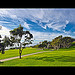
\includegraphics[height=0.2\textheight]{landscape.jpg} $\rightarrow$ 'landscape' \\
    
    
\includegraphics[height=0.2\textheight]{headshot.jpg} $\rightarrow$ 'headshot'
    \vskip20pt
    \normalsize
    e.g. determine if an image is a landscape or headshot
    }

  \end{center}

\end{frame}


\begin{frame}
  \frametitle{Classifying images}

  \begin{center}
    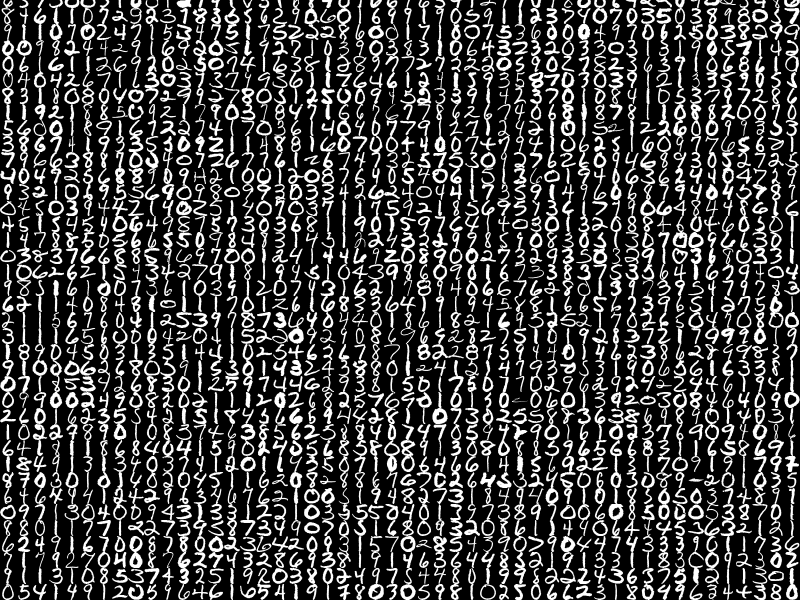
\includegraphics[width=0.75\textwidth]{../../code/image_data/sample_digits.png}
  \end{center}

\end{frame}
